\section{Results}
% TODO edit here
%%%% begin table----------------------------------------------
\begin{table*}
%\scriptsize %The standard font size switches are: \tiny, \scriptsize,  \footnotesize, \small, \normalsize, \large, \Large, \LARGE, \huge, and \Huge.
\centering
%\captionsetup{font=normal}
\footnotesize{\small}   
\resizebox{\textwidth}{!}{%
\begin{tabular}{|c|c|c|c|c|c|c|}
\hline 
&\multirow{2}*{} & \multicolumn{5}{c|}{{\bf Electron Binding Energy (cm$^{-1}$)} }\\
\cline {3-7}
& {\bf Dipole Moment (D)} & {\bf Experiment} & {\bf $\Delta$SCF\textsuperscript{\emph{a}}} & {\bf CCSD(T)\textsuperscript{\emph{a}}} & {\bf DMC\textsuperscript{\emph{b}}} & {\bf C-AFQMC\textsuperscript{\emph{c}}}\\ 
\hline % exp-dipole citation has no doi
{\bf SO} &1.55\cite{exp-dipole} &NOT-BOUND &-3.84  &-4.13 &-308.20 $\pm$ 70.82 &-4.54 $\pm$ 0.64\\
\hline
{\bf HCN} &2.98\cite{exp-dipole} &13\cite{10.1016/j.cplett.2009.04.007} &11.00 &7.44 &46.17 $\pm$ 45.30 &10.80 $\pm$ 2.95\\
\hline
{\bf CH$_2$CHCN}  &3.87\cite{exp-dipole} &56 - 87\cite{10.1103/PhysRevLett.73.2436,10.1103/PhysRevA.51.3667} &43.30 &61.87 &106.63 $\pm$ 58.12 &65.70 $\pm$ 11.03 \\
\hline
{\bf CH$_3$CN} &3.92\cite{exp-dipole} &93 - 145\cite{10.1103/PhysRevLett.73.2436,10.1103/PhysRevA.51.3667} &50.83 &103.00 &93.83 $\pm$ 36.21 &95.85 $\pm$ 9.73 \\
\hline
{\bf C$_3$H$_2$} &4.14\cite{10.1063/1.465007} &170 $\pm$ 50\cite{10.1063/1.472879} &54.61 &162.08 &151.22 $\pm$ 64.25\textsuperscript{\emph{d}} &132.45 $\pm$ 9.43\textsuperscript{\emph{e}}\\
\hline
{\bf C$_3$H$_2$O$_3$} &4.55\cite{exp-dipole} &194 $\pm$ 24\cite{10.1063/1.1629669} &103.13 &163.31 &213.98 $\pm$ 116.15 &157.70 $\pm$ 17.96 \\
\hline
\end{tabular}}
\caption{EBEs and dipole moments of selected species from experiment and Self-Consistent Field [HF], Coupled Cluster [CCSD(T)], DMC, and C-AFQMC calculations.}
\textsuperscript{\emph{a}} HF and CCSD(T) calculations were preformed using Gaussian 09.
\textsuperscript{\emph{b}} DMC calculations of the anion are based on unrestricted Hartree Fock (UHF) trial wave functions obtained from Gaussian 09 or GAMESS.
\textsuperscript{\emph{c}} AFQMC calculations were based on UHF trial wave functions obtained from NWChem.
\textsuperscript{\emph{d}} The DMC calculations on the C$_{3}$H$_{2}$ dipole-bound anion used a restricted open-shell Hartree Fock (ROHF) trial wave function.
\textsuperscript{\emph{e}} To be consistent, the C-AFQMC calculations on the C$_{3}$H$_{2}$ dipole-bound anion were also based on an ROHF trial wave function. 
\label{t1}
\end{table*}
%%%% end table----------------------------------------------
While DMC has been successfully employed to calculate cluster binding energies,\cite{10.1021/jp9066108,10.1021/jp404541c} here we analyze its performance predicting the electron binding energies of molecular dipole-bound anions. As an initial test, we examined whether DMC could faithfully predict whether a given species binds an extra electron or not. Thus, in addition to considering several species known to form dipole-bound anions, we also consider SO, a molecule with a dipole moment of 1.55 D, which is below the threshold required for binding. Our results are summarized in Table \ref{t1}. DMC calculations correctly predicted that all of the species studied, except SO, would form dipole-bound anions. 

In Figure \ref{f1}, the charge densities of neutral CH$_{3}$CN, the CH$_{3}$CN anion, and the SO molecule plus an extra electron are compared. While the DMC charge density for the neutral CH$_{3}$CN molecule is highly localized in the molecular region, that of the anion is far more diffuse and protrudes continuously out from the positive side of the dipole. The charge density plots of the other dipole-bound anions considered in this work manifest similar features and are reported in the Supplemental Information. In stark contrast, the charge density of SO plus an extra electron consists of two disjoint contributions -- one associated with the neutral molecule and a second representative of an additional unbound electron positioned more than 50 $\mbox{\AA}$ from the molecule. 
%%%% begin figure-----------------------------------------
\begin{center}
\begin{figure}[htbp]
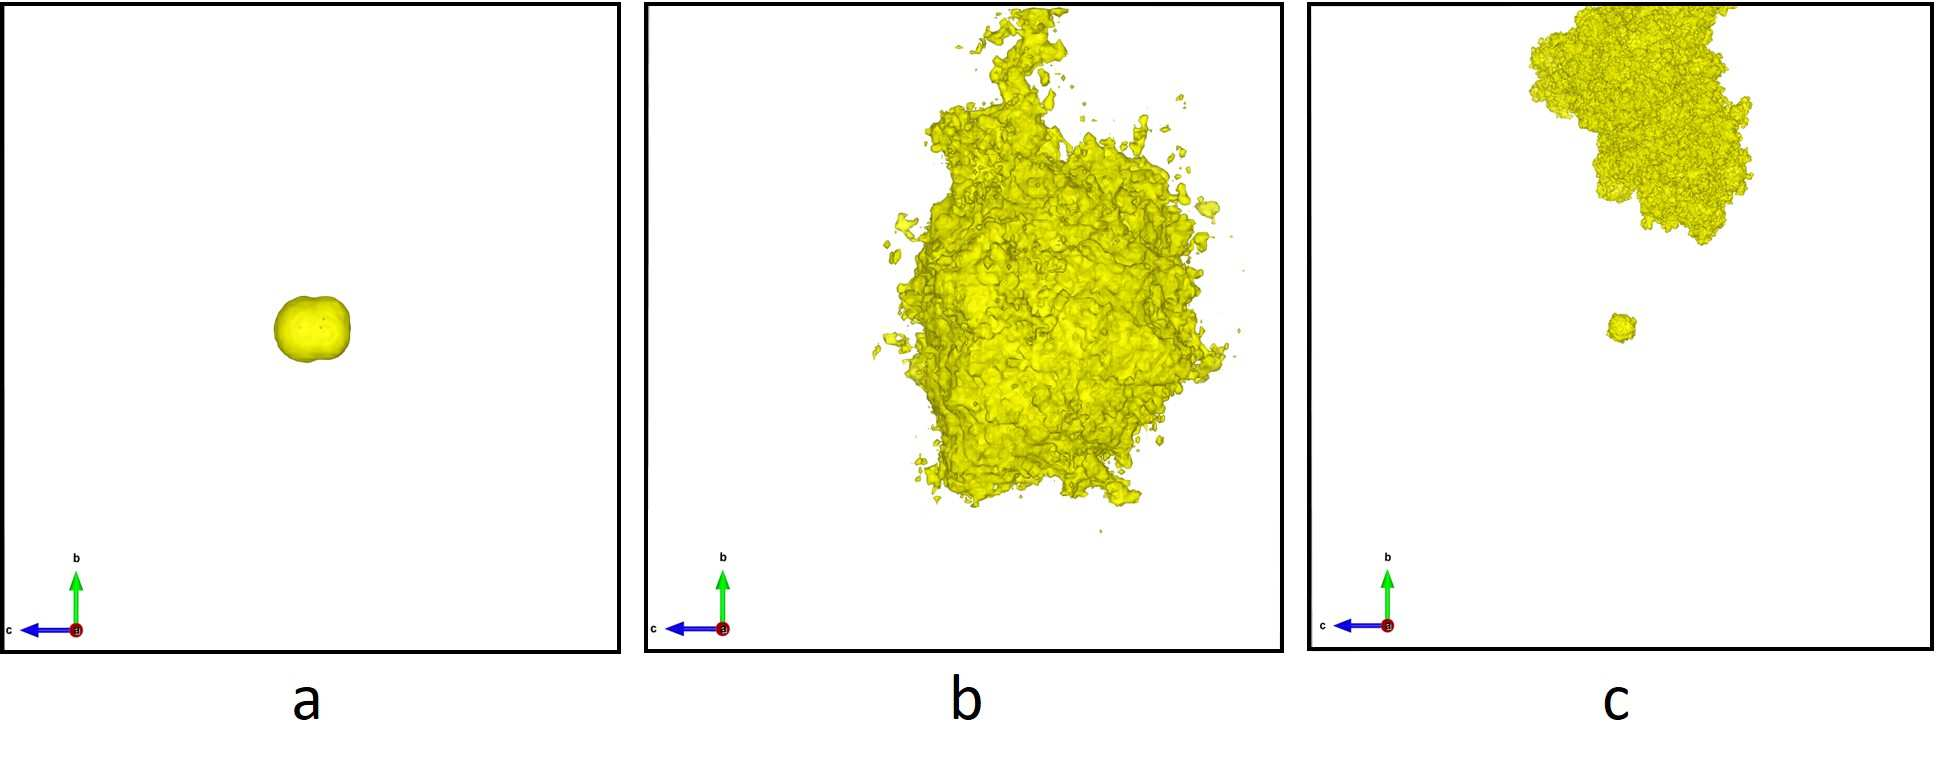
\includegraphics[width=\textwidth]{Images/chapter2/Neutral-anion-SO.pdf}
%\captionsetup{font=footnotesize, justification=raggedright, singlelinecheck=false}
\caption{DMC charge densities of (a) neutral CH$_3$CN, (b) the CH$_3$CN anion, and (c) SO plus an extra electron. The isosurface values taken for each of these plots are $4 \times 10^{-14}$ e/$\mbox{\AA}^3$, $4\times 10^{-14}$ e/$\mbox{\AA}^3$, and $1 \times 10^{-20}$ e/$\mbox{\AA}^3$, respectively. Molecules are placed in the center of the simulation box.}
\label{f1}
\end{figure}
\end{center}
%%%% end figure------------------------------------------

Interestingly, even though the fixed-node error in the energies of the neutral and anion are greater in magnitude than the electron binding energy, DMC calculations using  single Slater determinant trial wave functions provide semi-qualitatively accurate EBEs of dipole-bound anions. Nevertheless, obtaining quantitatively accurate EBEs with the DMC approach employed here would be too computationally demanding to be practical. As presented in Table \ref{t1}, achieving DMC statistical error bars smaller than the binding energies can require hundreds of thousands to millions of DMC iterations, even starting from a well-optimized variational wave function. For example, as depicted in Figure \ref{f2}, statistical fluctuations in the energy of the CH$_{3}$CN anion simulated with 4650 walkers hover around 65000 cm$^{-1}$, meaning that over 500,000 samples must be taken to achieve on the order of 100 cm$^{-1}$ error bars. Thus, while DMC EBEs that agree with experimental measurements and coupled cluster calculations can be gleaned from the noise, it is only with error bars that are still too large to make definitive statements and at great computational expense.
%%%% begin figure----------------------------------------------
\begin{center}
\begin{figure}[htbp]
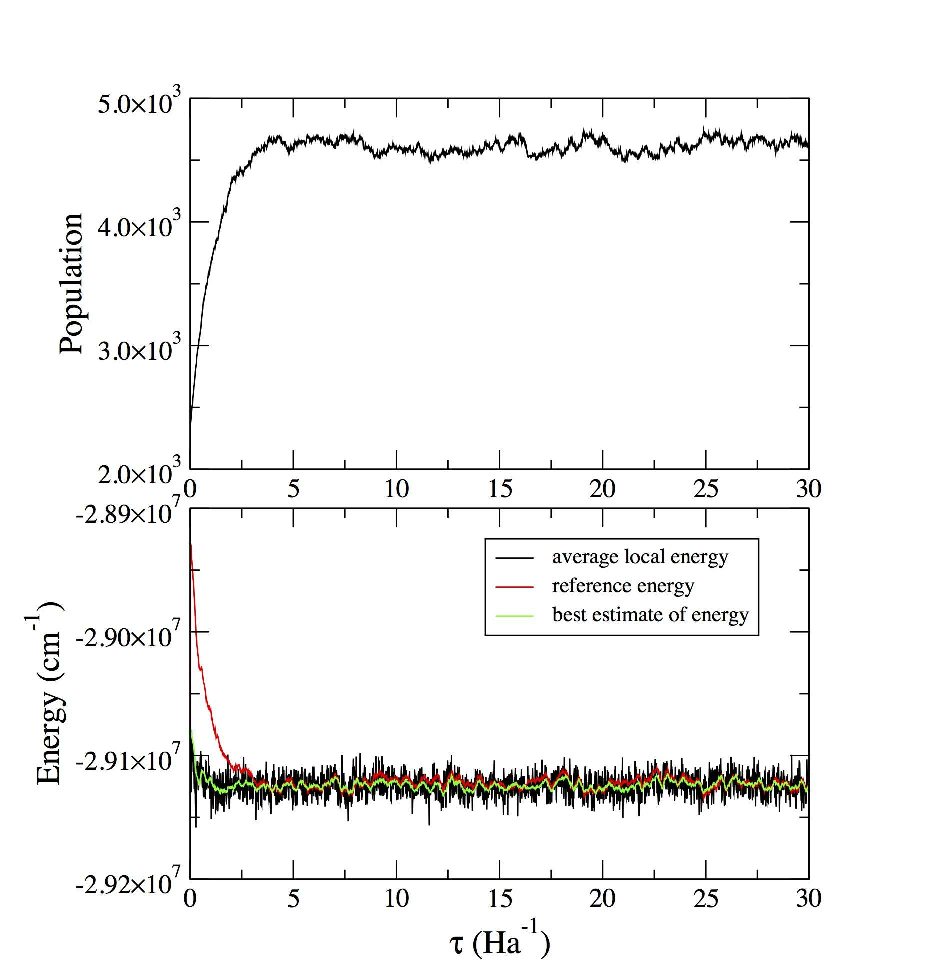
\includegraphics[width=\textwidth]{Images/chapter2/DMC-4.pdf}
%\captionsetup{font=footnotesize, justification=raggedright, singlelinecheck=false}
\caption{The time evolution of the DMC energy and walker population for the CH$_{3}$CN anion using $\Delta \tau = 0.01$ a.u. with 4650 walkers. Walkers were initialized with a UHF trial wave function expanded in terms of the aug-cc-pVDZ basis with a 7$s$7$p$ set of diffuse gaussian-type orbitals. In the Figure, reference energy refers to $E_{T}$ (see Supplemental Information), the average local energy refers to the local energy averaged over walkers at a given imaginary time, and best estimate of the energy refers to the energy averaged over all samples taken up to a certain imaginary time.}
\label{f2}
\end{figure}
\end{center}
%%%% end figure---------------------------------------------- 
\begin{center}
\begin{figure*}[htbp]
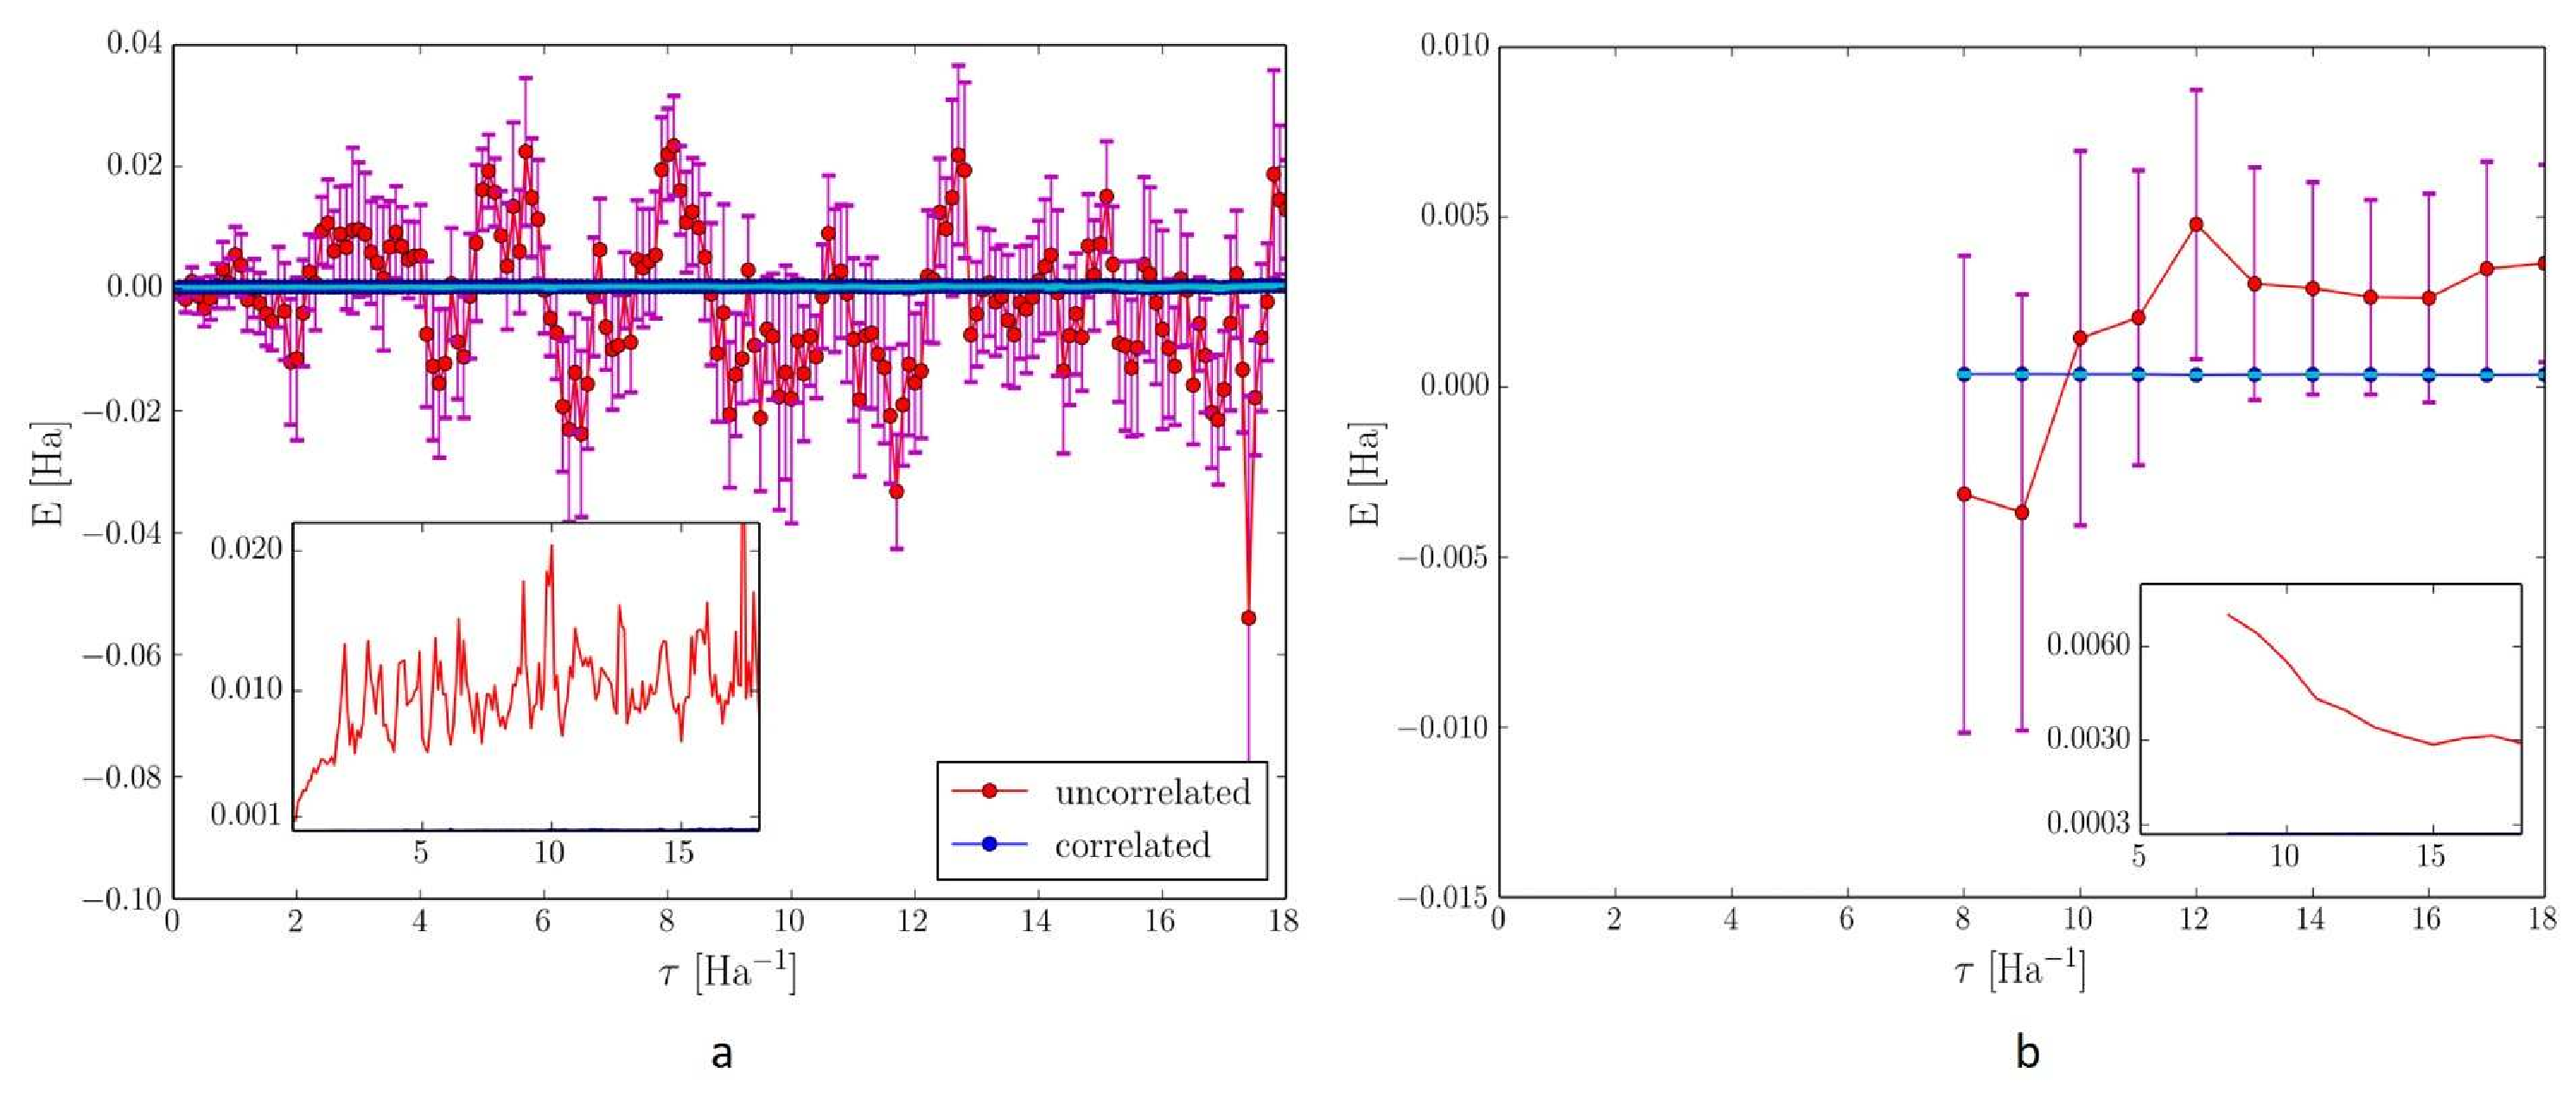
\includegraphics[width=\textwidth]{Images/chapter2/correlated_sampling.pdf}
%\captionsetup{font=footnotesize, justification=raggedright, singlelinecheck=false}
\caption{Comparison of energies from AFQMC calculations with and without correlated sampling for CH$_{3}$CN using the aug-cc-pvdz+7$s$7$p$ basis, an HF reference wave function, $\Delta \tau=0.01$ a.u., 384 walkers per simulation, and 17 repeated simulations. (a) Mean values of the EBE (circles) among the repeats at each $\tau$ along the imaginary-time propagation; (b) Mean values of the cumulative averages taken for $\tau > 8$ a.u. The error bars give the standard errors, defined as the standard deviation times $\frac{1}{\sqrt[]{N_r}}$, where $N_r$ is the number of simulation repeats, and are plotted in the insets for clarity.}
\label{f3}
\end{figure*}
\end{center}
%%%% end figure----------------------------------------------
One stochastic technique capable of scaling to dipole-bound anions of large molecules with a substantial reduction in statistical noise is C-AFQMC. As shown in Table \ref{t1}, C-AFQMC error bars are at least an order of magnitude smaller than DMC error bars using
a similar number of samples, but using two orders of magnitude shorter projection time (2000 a.u. was used to obtain most DMC results; 20 a.u. was used to obtain the C-AFQMC results). The C-AFQMC results presented were moreover obtained starting from just HF wave functions. One might question whether the source of this improvement stems from the AFQMC algorithm or from the use of correlated sampling. Figure \ref{f3}, which depicts the energy as a function of imaginary projection time for the CH$_{3}$CN molecule, demonstrates that the improvement may be attributed to \textit{both} sources. Uncorrelated AFQMC simulations are accompanied by statistical fluctuations on the order of $10^{4}$ cm$^{-1}$, which are smaller than the $10^{5}$ cm$^{-1}$ fluctuations associated with the EBE values from the DMC simulations (see Figure \ref{f2}). C-AFQMC calculations are accompanied by almost imperceptible statistical fluctuations on the order of 22 cm$^{-1}$. Thus, AFQMC's sampling innovations yield meaningful gains above DMC, yet it is the use of correlated sampling that yields, \textit{by far}, the largest improvements. 

As shown in Table \ref{t1}, C-AFQMC yields energies with sufficiently small error bars that meaningful comparisons can now be made against coupled cluster calculations and experiment. In general, the EBEs predicted by C-AFQMC are within error bars of both experimental and previous coupled cluster single, doubles, and perturbative triples (CCSD(T)) calculations. This demonstrates that phaseless approximation errors are mild and that for dipole-bound anions AFQMC is as accurate as CCSD(T). The C$_{3}$H$_{2}$ anion, however, stands as one cautionary tale. For the C$_{3}$H$_{2}$ anion, we located two different UHF solutions, neither of which proved suitable for trial functions in QMC calculations (see the
Supplemental Information for more details). For this reason, we employed an ROHF trial wave function for the C$_{3}$H$_{2}$ anion instead. This example suggests that care must be taken when selecting trial wave functions for and ultimately simulating larger molecules that may have many competing low-lying states.
